%Copyright 2014 Jean-Philippe Eisenbarth
%This program is free software: you can 
%redistribute it and/or modify it under the terms of the GNU General Public 
%License as published by the Free Software Foundation, either version 3 of the 
%License, or (at your option) any later version.
%This program is distributed in the hope that it will be useful,but WITHOUT ANY 
%WARRANTY; without even the implied warranty of MERCHANTABILITY or FITNESS FOR A 
%PARTICULAR PURPOSE. See the GNU General Public License for more details.
%You should have received a copy of the GNU General Public License along with 
%this program.  If not, see <http://www.gnu.org/licenses/>.

%Based on the code of Yiannis Lazarides
%http://tex.stackexchange.com/questions/42602/software-requirements-specification-with-latex
%http://tex.stackexchange.com/users/963/yiannis-lazarides
%Also based on the template of Karl E. Wiegers
%http://www.se.rit.edu/~emad/teaching/slides/srs_template_sep14.pdf
%http://karlwiegers.com
\documentclass{scrreprt}
\usepackage{listings}
\usepackage{underscore}
\usepackage[bookmarks=true]{hyperref}
\usepackage[utf8]{inputenc}
\usepackage[english]{babel}
\usepackage{graphicx}
\graphicspath{{./img/}}
\def\myversion{1.0 }
\date{}
%\title
\usepackage{hyperref}
\begin{document}

\begin{flushright}
    \rule{16cm}{5pt}\vskip1cm
    \begin{bfseries}
        \Huge{SOFTWARE REQUIREMENTS\\ SPECIFICATION}\\
        \vspace{1.9cm}
        for\\
        \vspace{1.9cm}
        Sports League Administration Manager (SLAM)\\
        \vspace{1.9cm}
        Prepared by Matt Strapp\\
        \vspace{1.9cm}
        University of Minnesota\\
        \vspace{1.9cm}
        \today\\
    \end{bfseries}
\end{flushright}

\tableofcontents


\chapter{Introduction}

\section{Purpose}

The purpose is to provide a description for the Sports League Administration Manager (SLAM). It will explain the purposes, features, interfaces, and designed use cases for the system. This is intended for both the Minneapolis Parks and Recreation Board and the developers of the service.

\section{Document Conventions}

This Document made to comply with the IEEE Software Requirements Format.

\section{Intended Audience and Reading Suggestions}
This document is designed to be read by the developers creating and maintaining SLAM, the administrators at the Minneapolis Parks and Recreation Board, and the athletes, league administrators, coaches, and other interested parties.

\section{Project Scope}
SLAM will be used by Minneapolis Municipal Parks and Recreation to organize sports leagues throughout the city. The system will provide methods for creating, managing, and administering sports leagues as well as assign officials. The system will also allow coaches to create teams and add players to teams.


\section{References}
\noindent
Sports League Administration Manager (SLAM) Software Requirements \\
\noindent
Sports League Administration Manager (SLAM) Use Cases

\chapter{Overall Description}

\section{Product Perspective}
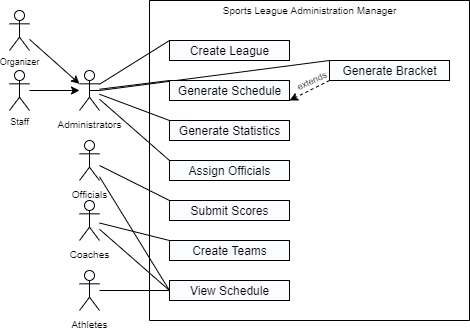
\includegraphics[width=\textwidth]{diagram} \\

The Sports League Administration Manager is developed to organize a 
$<$Describe the context and origin of the product being specified in this SRS.  
For example, state whether this product is a follow-on member of a product 
family, a replacement for certain existing systems, or a new, self-contained 
product. If the SRS defines a component of a larger system, relate the 
requirements of the larger system to the functionality of this software and 
identify interfaces between the two. A simple diagram that shows the major 
components of the overall system, subsystem interconnections, and external 
interfaces can be helpful.$>$

\section{Product Functions}
$<$Summarize the major functions the product must perform or must let the user 
perform. Details will be provided in Section 3, so only a high level summary 
(such as a bullet list) is needed here. Organize the functions to make them 
understandable to any reader of the SRS. A picture of the major groups of 
related requirements and how they relate, such as a top level data flow diagram 
or object class diagram, is often effective.$>$

\section{User Classes and Characteristics}
The system is divided into four users: administrators, officials, coaches, and the public. The roles are defined below.
\begin{itemize}
    \item Administrators:
    \begin{itemize}
        \item Create and manage leagues
        \item Create and manage league and tournament schedules 
        \item Generate user statistics on demand
        \item Assign officials to leagues and games
    \end{itemize}
\end{itemize}
Administrators include Staff members and the Parks and Recreation Organizer.  They have the highest privilege level. Administrators are the ones in charge of creating leagues, scheduling games, and assigning officials. They also are the users that create statistics and deal with finances.
\begin{itemize}
    \item Officials:
    \begin{itemize}
        \item Submit their availability to official games
        \item Accept or reject games to officiate
        \item View the schedule of games they need to attend
        \item Submit scores when game is complete
    \end{itemize}
\end{itemize}
Officials are responsible for submitting scores when games are over. They also are responsible for submitting their schedules so all games played have a sufficient number of officials.
\begin{itemize}
    \item Coaches:
    \begin{itemize}
        \item Create teams
        \item Add athletes to teams
    \end{itemize}
\end{itemize}
Coaches are responsible for creating teams and adding athletes to teams.
\begin{itemize}
    \item Athletes, the Public:
    \begin{itemize}
        \item View schedule
    \end{itemize}
\end{itemize}
Athletes and other end users need to be able to view the schedule of games they plan on attending or playing in.

\section{Assumptions and Dependencies}

It is assumed that an external database and interface already exist.

\chapter{System Features}

\section{League Creation}

\subsection{Description and Priority}
The system shall allow administrators to create leagues for sports. The system will list sports to create a league for and the user will select the sport. The system will then list the leagues that are available for the sport and the user will select the league.

\subsection{Stimulus/Response Sequences}
A user must be logged in as an administrator to be able to create a league. The user submits the sport they want to create a league for and the system will respond by verifying the response and creating a new league if the response is valid.

\subsection{Functional Requirements}
REQ-101: The system shall list all sports that leagues can be created for. \\
REQ-102: The system shall validate the user input. \\
REQ-103: The system shall return an error if the user tries to create a league for a sport that does not exist or is no longer allowing league creation. \\
REQ-104: The system shall create the league after verifying the input. \\
\indent Valid sports are as follows: Sand Volleyball, Kickball, Indoor Soccer, Softball, Outdoor Soccer, Tennis, Flag Football, Fall Soccer, Dodgeball, Indoor Volleyball, Fall Kickball, Fall Softball, Basketball, Broomball, and Pond Hockey.


\section{Schedule Generation}

\subsection{Description and Priority}
The system shall allow administrators to create schedules for leagues.

\subsection{Stimulus/Response Sequences}
A user must be signed in as an administrator. The user supplies a beginning and ending date for the schedule and the system will generate a schedule for the league.

\subsection{Functional Requirements}

REQ-201: The user must specify a start and end date for the league. \\
REQ-202: The system shall verify the dates. The verification process is TBD.
REQ-203: The system shall generate a valid schedule for the league provided between the dates provided. The verification process for this is TBD.\\
REQ-204: The system shall return an error if the dates are invalid. \\
REQ-205: The system shall return an error if it cannot generate a schedule for the league.
REQ-206: The system shall return a valid generated schedule after it has validated the inputs. What constitutes a valid schedule is TBD. \\

\section{Team Creation}
    
    \subsection{Description and Priority}   
    The system shall allow coaches and administrators to register teams.
    \subsection{Stimulus/Response Sequences}    
    A user must be signed in as a coach or administrator. The user supplies the name of the team and the system will create the team. The user must supply a valid roster and the league they want to register the team for.
    \subsection{Functional Requirements}
    REQ-301: The system shall validate the number of team members and return an error if the team is too small for the sport. \\
    REQ-302: The system shall validate the team name and return an error if the team name is invalid. What constitutes an invalid team name is TBD. \\
    REQ-303: The system shall create a team with the supplied roster and name and add it to the database.

\section{Roster Editing}
  
    \subsection{Description and Priority}   
    The system shall allow coaches and administrators to edit rosters.
        \subsection{Stimulus/Response Sequences}    
    A user must be signed in as a coach or administrator. The user submits the change that they want to make to the roster. The system responds by changing the roster as requested.
        \subsection{Functional Requirements}
    REQ-401: The system shall return an error if the user does not have permission to edit that team's roster. \\
    REQ-402: The system shall return an error if the user tries to edit a team that does not exist. \\
    REQ-403: The system shall change the roster as requested if the user has permission to edit that team's roster.
\section{Generate Statistics}

    \subsection{Description and Priority}
    The system shall allow administrators to generate statistics.
    \subsection{Stimulus/Response Sequences}
    A user must be signed in as an administrator. The user submits the type of statistics they want to generate. The system will generate the statistics asked.
    \subsection{Functional Requirements}
    REQ-501: The system shall return an error if the user tries to generate statistics for a sport, league or player that does not exist. \\
    REQ-502: The system shall generate the statistics and display them to the user when generated.

\section{Assign Officials}
    \subsection{Description and Priority}
    The system shall allow administrators to assign officials to leagues and games.
    \subsection{Stimulus/Response Sequences}
    A user must be signed in as an administrator. The user submits the league and game they want to assign officials to. The system will assign the officials to the game based on the schedule given by the officials.
    \subsection{Functional Requirements}
    REQ-601: The system shall return an error if the user tries to assign officials to a league or game that does not exist. \\
    REQ-602: The system shall return an error if no officials can be found for a game. \\
    REQ-603: The system shall assign the officials to the game and publish the schedule so the officals can see what games they need to officiate.

\section{Submit Scores}
    \subsection{Description and Priority}
    The system shall allow officials to submit scores for games they officiate.
    \subsection{Stimulus/Response Sequences}
    A user must be signed in as an official. The user submits the score for the game they are officiating.
    \subsection{Functional Requirements}
    REQ-701: The system shall return an error if the user tries to submit a score for a game that does not exist. \\
    REQ-702: The system shall return an error if the user tries to submit a score for a game that is not officiating. \\
    REQ-703: The system shall submit the score to the database and publish it to an external site after the submission is complete. \\
    REQ-704: The system shall allow administrators to change scores if they contradict the official's reported scores.

    
    \section{Generate Bracket}
    \subsection{Description and Priority}
    The system shall allow administrators to generate brackets for leagues.
    \subsection{Stimulus/Response Sequences}
    A user must be signed in as an administrator. The user submits the league they want to generate a bracket for. The system will generate the bracket along with the dates for the games. \\
    This requirement is built off of requirement 2.
    \subsection{Functional Requirements}
    REQ-801: The system shall return an error if the user tries to generate a bracket for a league that does not exist. \\
    REQ-802: The system shall generate the bracket and proceed to generate the schedule according to Requirement 2. \\
    REQ-803: The system shall return an error if the system cannot generate the bracket requested. \\
    
    \section{View Schedules}
    \subsection{Description and Priority}
    The system shall allow users to view schedules for leagues.
    \subsection{Stimulus/Response Sequences}
    Any user can access the schedule for a league. They do not have to be signed in to view the public schedules. Officals can view the schedule for a league they are officiating and administrators can view any schedule for any league.
    \subsection{Functional Requirements}
    REQ-901: The system shall return an error if the user tries to view a schedule for a league that does not exist. \\
    REQ-902: The system shall return an error if an unauthenticated user tries to view a schedule for a league that is not public. \\
    REQ-903: The system shall return an error if an authenticated user tries to view a schedule for a league that they do not have permission to access. \\
    REQ-904: The system shall return the schedule for the league requested.


\section{Appendix A: Glossary}
%see https://en.wikibooks.org/wiki/LaTeX/Glossary
SLAM: The Sports League Administration Manager
Staff: The people who run the league, working for the Municipal Parks and Recreation Department.
Administrators: People with administrative privileges.
Officals: People who officiate games.
Coaches: People who create teams.
Athletes: People who play in the leagues.
The Public: Everyone else.


\section{Appendix B: To Be Determined List}
TODO: specifications, testing, the rest of the document
\end{document}